% Provenance (never printed): old premiere S material on the formation of fossil
% fuels (preserved organic matter, burial, oil window, migration, trap, coal).
% Burial history of the invented Merrow Basin from figdata/grade-11/oil_window.py
% (constant geotherm, no compaction). Rifts and passive margins after the USGS
% West-Central Coastal Province fact sheet (2023-3028). Folds are defined in
% g12.02 mountain-building (Sync 0): the anticline is told in prose here, never
% defined. Sedimentary basins compared, diagenesis: Year 1/2.
\chapter{جيولوجيا الفحم والنفط والغاز}\label{ch:g11:fossil-fuel-geology}

لوح من السجيل الأسود أُخذ من منجم \omterm{def:g11:fossil-fuel-geology:coal}{فحم} قديم في بنسلفانيا يحمل
أوراق نباتات شبيهة بالسرخس، مسطحة فضية اللون على الصخر الداكن. وقد
نمت في مستنقع قبل أكثر من ثلاثمئة مليون سنة، في
العصر الكربوني؛ ولأنها دُفنت قبل أن تتعفن، احتفظت بشكلها، وصار
كربون نباتات المستنقع فحمًا. والنفط والغاز، اللذان يُضخّان اليوم من
منصات في عرض البحر، لهما أصل من النوع نفسه: بقايا كائنات
حية أفلتت من التحلل ثم دُفنت وسُخّنت. يتتبع هذا الفصل
ذلك الكربون المدفون من المستنقع وقاع البحر إلى طبقة \omterm{def:g11:fossil-fuel-geology:coal}{الفحم}
وحقل النفط.
% ledger: photo:g11-fossil-plants, ics:base.Carboniferous, ics:base.Permian, earle:coal-formation, earle:organic-preservation

\begin{omfigure}
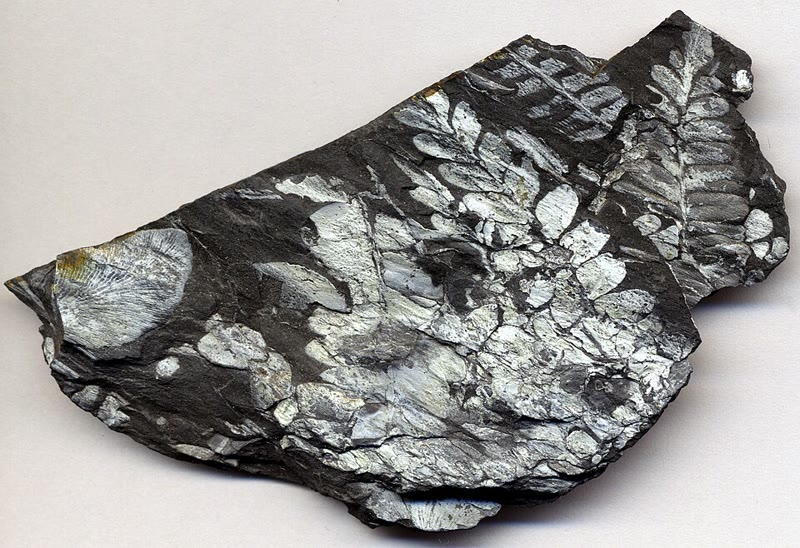
\includegraphics[height=4.4cm]{images/book2/g11-stjohn-fossil-plants.jpg}\hspace{0.03\linewidth}%
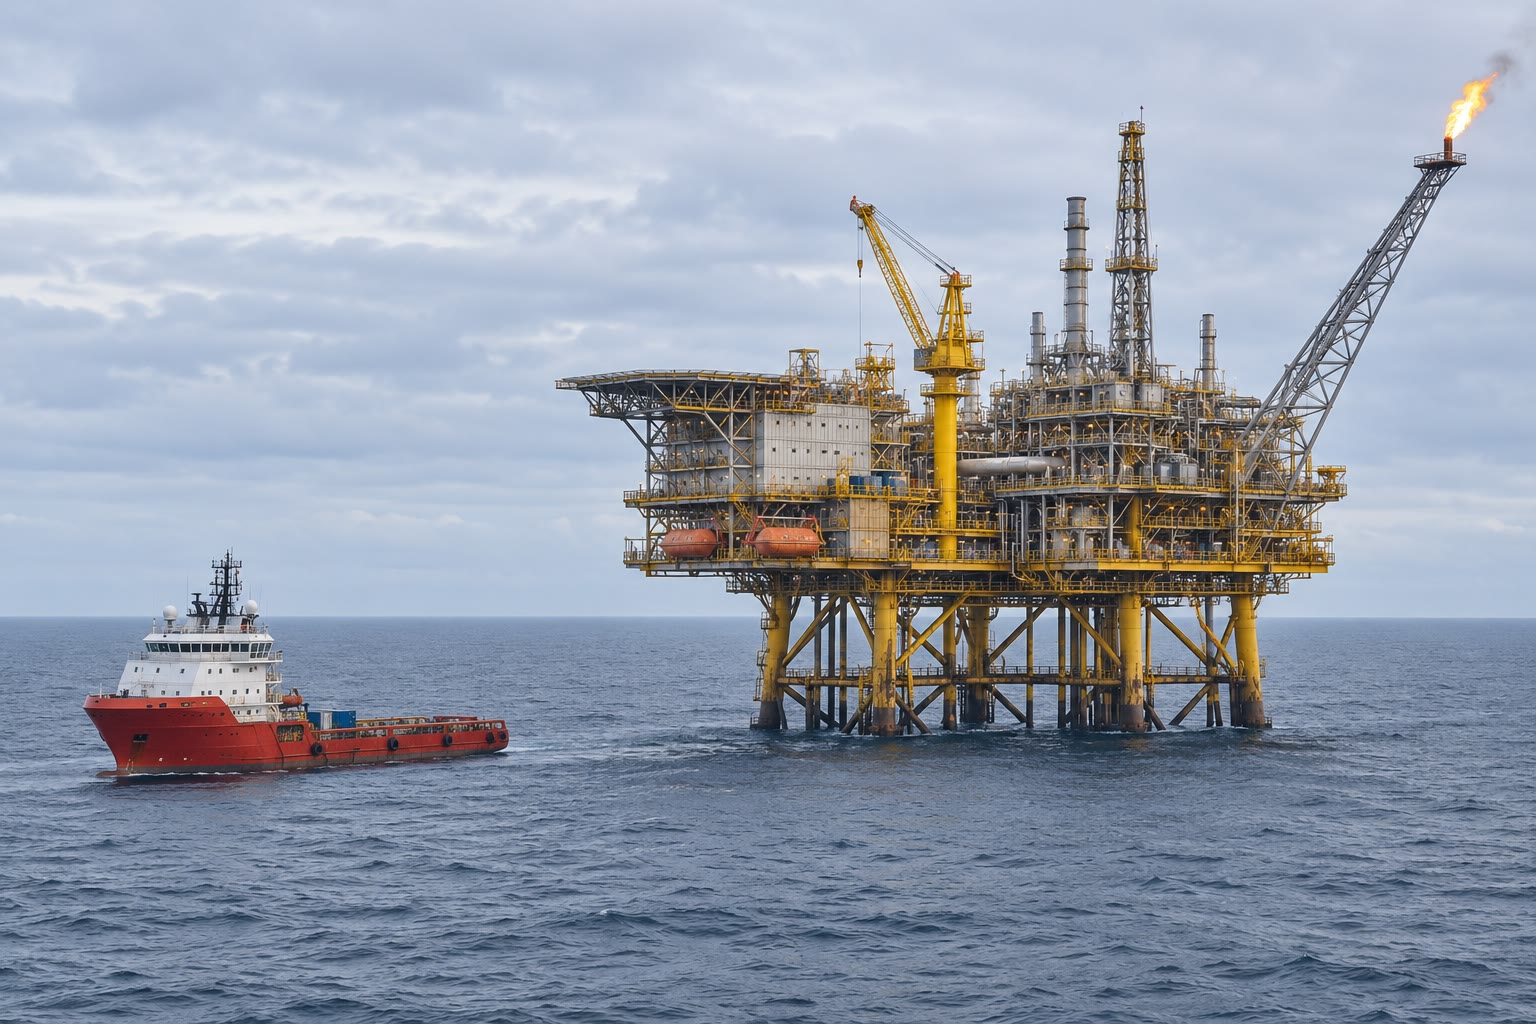
\includegraphics[height=4.4cm]{images/book2/ai/g11-offshore-platform.jpg}

{\small في اليمين: أوراق نباتات أحفورية في سجيل غني بالكربون من منجم
\omterm{def:g11:fossil-fuel-geology:coal}{فحم} قديم، بنسلفانيا، العصر الكربوني؛ عرض اللوح نحو \qty{10}{cm}.
الصورة: جيمس سانت~جون (\babelsublr{CC~BY~2.0}). في اليسار: منصة لإنتاج
النفط والغاز في البحر (رسم مولَّد بالذكاء الاصطناعي).}
\end{omfigure}
% ledger: photo:g11-fossil-plants

\begin{recall}
\omterm{def:g11:fossil-fuel-geology:coal}{الفحم} والنفط والغاز الطبيعي أنواع من الوقود الأحفوري: فالنفط والغاز مزيجان من
الهيدروكربونات، وهي مركبات من الكربون والهيدروجين، واحتراق الوقود الأحفوري
يطلق الطاقة وثنائي أكسيد الكربون (كتب الكيمياء). والنباتات والطحالب
تصنع المادة العضوية من ثنائي أكسيد الكربون والماء بالتركيب الضوئي (كتب
الأحياء). \omterm{def:g11:fossil-fuel-geology:coal}{والفحم} والنفط والغاز تأتي من مادة عضوية دُفنت في
الرواسب، وهي مخزونة في الصخور الرسوبية (الكتاب 1، الصف 9). والصخر
مسامي حين تكون فيه فراغات، ونفوذ حين يستطيع الماء الجريان عبره
(الكتاب 1، الصف 6). وترتفع درجة الحرارة مع العمق على امتداد \omterm{def:g11:lithosphere-asthenosphere:geotherm}{المنحنى الحراري الأرضي}،
بمقدار 25 إلى \qty{30}{\degreeCelsius} لكل كيلومتر في الكيلومترات الأولى
(\cref{ch:g11:lithosphere-asthenosphere}).
\end{recall}
% ledger: usgs:gradient-29, earle:organic-preservation

\section{حفظ المادة العضوية}

معظم المادة العضوية لا يصير وقودًا أبدًا. فالورقة الميتة أو الطحلب الميت
تأكله الحيوانات والبكتيريا أو يتفاعل مع أكسجين الهواء: وفي غضون
أسابيع أو سنوات يكون كربونه قد عاد إلى الغلاف الجوي ثنائيَ أكسيد كربون.
ولا تبقى المادة العضوية إلا حيث تُعزل عن الأكسجين --- في
قاع مستنقع راكد، أو على قاع بحر أو قاع بحيرة لا يحوي ماؤه
أكسجينًا. وإذا دُفنت هناك تحت مزيد من الرواسب، أمكن أن تُحفظ عشرات أو
مئات الملايين من السنين.
% ledger: earle:organic-preservation

يأتي \omterm{def:g11:fossil-fuel-geology:coal}{الفحم} في معظمه من نباتات برية تراكمت في المستنقعات. ويأتي النفط والغاز
في معظمهما من الطحالب المجهرية وغيرها من عوالق البحر: فحيث تكون
المياه السطحية شديدة الإنتاجية، تتساقط العوالق الميتة على قاع البحر
بسرعة تكفي لينجو بعضها من التحلل، فيُدفن في الوحل.
% ledger: earle:coal-formation, earle:oil-window

\begin{definition}[الصخر المصدر؛ الكيروجين]\label{def:g11:fossil-fuel-geology:source-rock}
\emph{الكيروجين}\index{كيروجين} هو المادة العضوية المبعثرة في
صخر رسوبي، على هيئة جسيمات صغيرة لا تذوب في المذيبات
العضوية. و\emph{الصخر المصدر}\index{صخر مصدر} صخر رسوبي غني
بالكيروجين، يتكوّن فيه النفط والغاز حين يُدفن ويُسخَّن.
\end{definition}
% ledger: peters08:kerogen, earle:migration-traps

معظم الصخور المصدر من السجيل والحجر الطيني، ترسبت أوحالًا غنية
بالمادة العضوية. وقرب السطح يبقى كيروجينها صلبًا: فالبكتيريا التي تعيش
دون أكسجين تحوّل بعض المادة العضوية إلى ميثان، لكن معظم
ذلك الميثان يفلت عائدًا إلى السطح. وصنع النفط يحتاج إلى الحرارة، والحرارة تحتاج إلى العمق.
% ledger: earle:oil-window, peters08:kerogen

\section{الدفن والنضج}

\begin{definition}[الحوض الرسوبي]\label{def:g11:fossil-fuel-geology:basin}
\emph{الحوض الرسوبي}\index{حوض رسوبي} منطقة من القشرة
تهبط على مدى ملايين السنين، فتتراكم فيها الرواسب، وكثيرًا ما يبلغ سمكها
عدة كيلومترات.
\end{definition}
% ledger: usgs23:rift-salt

في حوض هابط، تُدفن كل طبقة أعمق فأعمق تحت الطبقات
التي تتراكم فوقها. وهي إذ تنزل تتبع \omterm{def:g11:lithosphere-asthenosphere:geotherm}{المنحنى الحراري الأرضي}: فهي
تُسخَّن. فيُطهى كيروجينها ببطء، وتنكسر جزيئاته الكبيرة إلى
جزيئات النفط والغاز الأصغر.
% ledger: earle:oil-window

\begin{definition}[النضج؛ نافذة النفط؛ نافذة الغاز]\label{def:g11:fossil-fuel-geology:oil-window}
\emph{نضج}\index{نضج (الصخر المصدر)} \omterm{def:g11:fossil-fuel-geology:source-rock}{الصخر المصدر} هو
تحول كيروجينه إلى نفط وغاز حين يُدفن ويُسخَّن.
و\emph{نافذة النفط}\index{نافذة النفط} هي مجال درجات الحرارة، من
نحو 60 إلى \qty{120}{\degreeCelsius}، الذي يكوّن فيه \omterm{def:g11:fossil-fuel-geology:source-rock}{الكيروجين} النفط في الغالب.
وفيما وراء نحو \qty{120}{\degreeCelsius}، في \emph{نافذة
الغاز}\index{نافذة الغاز}، يكوّن الميثان في الغالب.
\end{definition}
% ledger: earle:oil-window, magoon00:tps

لأن درجة الحرارة ترتفع مع العمق، فإن \omterm{def:g11:fossil-fuel-geology:oil-window}{نافذة النفط} هي أيضًا مجال من
الأعماق. وحيث يكون \omterm{def:g11:lithosphere-asthenosphere:geotherm}{المنحنى الحراري الأرضي} خطًا مستقيمًا، يسهل إيجادها.

\begin{proposition}[عمق نافذة النفط]\label{prop:g11:fossil-fuel-geology:window-depth}
لتكن درجة الحرارة $T_0$ عند السطح ولترتفع مع العمق $z$ \omterm{def:g11:lithosphere-asthenosphere:geotherm}{بتدرج
حراري أرضي} ثابت $G$: $T = T_0 + G z$. عندئذ تقع \omterm{def:g11:fossil-fuel-geology:oil-window}{نافذة النفط}
بين العمقين
\[
  z_{\text{أعلى}} = \frac{60 - T_0}{G}
  \qquad\text{و}\qquad
  z_{\text{قاعدة}} = \frac{120 - T_0}{G},
\]
ودرجات الحرارة بوحدة \unit{\degreeCelsius}. وسمكها $60/G$: فكلما
كان \omterm{def:g11:lithosphere-asthenosphere:geotherm}{المنحنى الحراري الأرضي} أشد انحدارًا، كانت النافذة أقل عمقًا وأرق.
\end{proposition}
% ledger: earle:oil-window

\begin{proof}
أعلى النافذة هو العمق الذي يكون عنده $T_0 + G z = 60$، أي
$z = (60 - T_0)/G$؛ والقاعدة حيث $T_0 + G z = 120$. والفرق هو
$(120 - 60)/G = 60/G$.
\end{proof}

إذا كان السطح عند \qty{20}{\degreeCelsius} والتدرج
\qty{30}{\degreeCelsius} لكل كيلومتر، فإن \omterm{def:g11:fossil-fuel-geology:oil-window}{نافذة النفط} تقع بين
$40/30 \approx \qty{1.3}{km}$ و$100/30 \approx \qty{3.3}{km}$. وفي الآبار
المحفورة في أنحاء الولايات المتحدة، يبلغ متوسط التدرج
\qty{29}{\degreeCelsius} لكل كيلومتر، و\num{25} في الشرق و\num{34}
في الغرب؛ وعادةً لا بد أن يُدفن \omterm{def:g11:fossil-fuel-geology:source-rock}{الصخر المصدر} أعمق من نحو
\qty{2}{km} قبل أن يصنع النفط. وحين لا يتوفر أي قياس \omterm{def:g11:fossil-fuel-geology:source-rock}{للكيروجين}،
اعتاد جيولوجيو النفط أن يعدّوا \omterm{def:g11:fossil-fuel-geology:source-rock}{الصخر المصدر} المدفون تحت أكثر
من نحو \qty{3}{km} من الصخور الأحدث ناضجًا.
% values (oil_window.py): z_top_km 1.3333, z_base_km 3.3333
% ledger: usgs:gradient-29, earle:oil-window, magoon00:tps

\begin{omfigure}
\begin{tikzpicture}
\begin{axis}[omrecord, omage, omdepth, name=burial, width=0.54\linewidth, height=5.6cm,
  xmin=0, xmax=170, ymin=0, ymax=4.5, xlabel={\foreignlanguage{arabic}{العمر بملايين السنين قبل الحاضر}},
  ylabel={\foreignlanguage{arabic}{العمق \babelsublr{(\unit{km})}}}, unbounded coords=jump, clip=false,
  xtick={0,20,...,160}, ytick={0,1,...,4}]
\fill[omProp!18] (axis cs:170,1.3333) rectangle (axis cs:0,3.3333);
\fill[omThm!12] (axis cs:170,3.3333) rectangle (axis cs:0,4.5);
\node[font=\scriptsize, anchor=west, text=omProp!80!black] at (axis cs:168,1.75) {نافذة النفط};
\node[font=\scriptsize, anchor=west, text=omThm] at (axis cs:168,3.9) {نافذة الغاز};
\node[font=\scriptsize, anchor=south west, text=black!60, inner sep=1pt] at (axis cs:168,1.3333) {\qty{60}{\degreeCelsius}};
\node[font=\scriptsize, anchor=south west, text=black!60, inner sep=1pt] at (axis cs:168,3.3333) {\qty{120}{\degreeCelsius}};
% computed in figdata/grade-11/oil_window.py (invented basin)
\addplot[black!45, line width=0.6pt] table[x=age, y=z150] {figdata/out/grade-11-oil_window-history.dat};
\addplot[black!45, line width=0.6pt] table[x=age, y=z120] {figdata/out/grade-11-oil_window-history.dat};
\addplot[black!45, line width=0.6pt] table[x=age, y=z95] {figdata/out/grade-11-oil_window-history.dat};
\addplot[black!45, line width=0.6pt] table[x=age, y=z66] {figdata/out/grade-11-oil_window-history.dat};
\addplot[black, line width=1.4pt] table[x=age, y=z165] {figdata/out/grade-11-oil_window-history.dat};
\draw[omDef, dashed, line width=0.8pt] (axis cs:80,0) -- (axis cs:80,4.5);
\node[font=\scriptsize, anchor=west, text=omDef, inner sep=1pt] at (axis cs:78,4.2) {تكوّن الطية المحدبة};
\fill[omThm] (axis cs:116.97,1.3333) circle (2pt);
\fill[omThm] (axis cs:51.24,3.3333) circle (2pt);
\node[font=\scriptsize, anchor=north east, inner sep=1pt] at (axis cs:100,2.3) {الصخر المصدر};
\end{axis}
\begin{axis}[omrecord, omdepth, at={(burial.east)}, anchor=west, xshift=1.7cm, width=0.34\linewidth, height=5.6cm,
  xmin=15, xmax=50, ymin=0, ymax=7, xlabel={\foreignlanguage{arabic}{التدرج \babelsublr{(\unit{\degreeCelsius/km})}}},
  ylabel={\foreignlanguage{arabic}{العمق \babelsublr{(\unit{km})}}}]
% computed in figdata/grade-11/oil_window.py (proposition, surface at 20 degC)
\addplot[name path=top, omProp, line width=1pt] table[x=G, y=z_top] {figdata/out/grade-11-oil_window-windows.dat};
\addplot[name path=base, omThm, line width=1pt] table[x=G, y=z_base] {figdata/out/grade-11-oil_window-windows.dat};
\addplot[omProp!18] fill between[of=top and base];
\node[font=\scriptsize] at (axis cs:40,1.75) {نافذة النفط};
\node[font=\scriptsize, anchor=south, text=omProp!80!black] at (axis cs:42,0.95) {الأعلى};
\node[font=\scriptsize, anchor=north west, text=omThm] at (axis cs:24,4.6) {القاعدة};
\end{axis}
\end{tikzpicture}

{\small في اليسار: تاريخ دفن حوض ميرو، وهو حوض مُتخيَّل (نموذج
محسوب، مع إهمال الانضغاط). يتتبع كل خط طبقة واحدة عبر الزمن، منذ
اليوم الذي ترسبت فيه على السطح؛ والخط السميك هو \omterm{def:g11:fossil-fuel-geology:source-rock}{الصخر المصدر}،
الذي ترسب قبل 165 مليون سنة. ومع سطح عند
\qty{20}{\degreeCelsius} وتدرج قدره \qty{30}{\degreeCelsius} لكل
كيلومتر، تكون \omterm{def:g11:fossil-fuel-geology:oil-window}{نافذة النفط} هي الشريط الواقع بين \num{1.3}
و\qty{3.3}{km}. وتحدد النقاط متى دخلها \omterm{def:g11:fossil-fuel-geology:source-rock}{الصخر المصدر} ومتى
غادرها إلى \omterm{def:g11:fossil-fuel-geology:oil-window}{نافذة الغاز}. في اليمين: عمق أعلى \omterm{def:g11:fossil-fuel-geology:oil-window}{نافذة النفط} وقاعدتها
بدلالة \omterm{def:g11:lithosphere-asthenosphere:geotherm}{التدرج الحراري الأرضي} (السطح عند
\qty{20}{\degreeCelsius}).}
\end{omfigure}
% values (oil_window.py): enter_oil_Ma 116.97, leave_oil_Ma 51.24, T_max 140 (20 Ma), T_today 125

يسمى مخطط كهذا \emph{مخطط تاريخ الدفن}: يجري فيه العمر من
اليسار إلى اليمين نحو اليوم، والعمق نحو الأسفل. وهو يحوّل عمودًا من الصخور،
مؤرخًا طبقة طبقة، إلى قصة.

\begin{method}[قراءة مخطط تاريخ الدفن]\label{met:g11:fossil-fuel-geology:burial}
\begin{enumerate}
  \item جد خط \omterm{def:g11:fossil-fuel-geology:source-rock}{الصخر المصدر}: إنه يبدأ عند السطح في
        اليوم الذي ترسب فيه الصخر.
  \item ارسم أعلى \omterm{def:g11:fossil-fuel-geology:oil-window}{نافذة النفط} وقاعدتها، بوصفهما عمقين، انطلاقًا من
        \omterm{def:g11:lithosphere-asthenosphere:geotherm}{المنحنى الحراري الأرضي} (\cref{prop:g11:fossil-fuel-geology:window-depth}).
  \item اقرأ العمر الذي يقطع عنده خط \omterm{def:g11:fossil-fuel-geology:source-rock}{الصخر المصدر} أعلى
        النافذة: عندئذ يبدأ \omterm{def:g11:fossil-fuel-geology:source-rock}{الصخر المصدر} بصنع النفط. واقرأ العمر الذي
        يقطع عنده القاعدة: ومنذئذ يصنع الغاز.
  \item قارن هذين العمرين بعمر \omterm{def:g11:fossil-fuel-geology:trap}{المصيدة}: فلا يمكن أن تحتجز \omterm{def:g11:fossil-fuel-geology:trap}{المصيدة} إلا النفط والغاز
        المتكونين بعد وجودها.
\end{enumerate}
\end{method}
% ledger: magoon00:tps

في حوض ميرو، يدخل \omterm{def:g11:fossil-fuel-geology:source-rock}{الصخر المصدر} \omterm{def:g11:fossil-fuel-geology:oil-window}{نافذة النفط} قبل نحو 117
مليون سنة ويغادرها قبل نحو 51 مليون سنة؛ ويبلغ أعمق
دفن له، \qty{4.0}{km} عند \qty{140}{\degreeCelsius}، قبل 20 مليون سنة،
قبل أن يرفعه النهوض والتعرية من جديد. وهو اليوم لا يزال في \omterm{def:g11:fossil-fuel-geology:oil-window}{نافذة
الغاز}. ومسألة نهاية الأسبوع تحسب هذه الأعمار.
% values (oil_window.py): enter_oil_Ma 116.97, leave_oil_Ma 51.24, z_max_km 4, T_max 140, T_today 125

\section{من المصدر إلى المصيدة}

النفط والغاز أخف من الماء، ومسام الصخور المدفونة مملوءة
بالماء. فما إن يتكوّنا حتى يُدفعا خارج \omterm{def:g11:fossil-fuel-geology:source-rock}{الصخر المصدر} ويزحفا إلى الأعلى،
عبر أي صخر يسمح بمرورهما.
% ledger: earle:migration-traps

\begin{definition}[الهجرة]\label{def:g11:fossil-fuel-geology:migration}
\emph{الهجرة}\index{هجرة (النفط والغاز)} هي الحركة البطيئة
للنفط والغاز خارج \omterm{def:g11:fossil-fuel-geology:source-rock}{الصخر المصدر} الذي تكوّنا فيه، صعودًا عبر
صخور نفوذة، تدفعهما كثافتهما الأقل من كثافة الماء المحيط بهما.
\end{definition}
% ledger: earle:migration-traps

\begin{definition}[الصخر الخازن؛ الصخر الحاجز]\label{def:g11:fossil-fuel-geology:reservoir}
\emph{الصخر الخازن}\index{صخر خازن} صخر مسامي ونفوذ
يتجمع فيه النفط والغاز: فمسامه تخزنهما، والوصلات بينها
تسمح لهما بالجريان نحو البئر. و\emph{الصخر الحاجز}\index{صخر حاجز} صخر
كتيم فوق الصخر الخازن، لا يستطيع النفط والغاز
عبوره.
\end{definition}
% ledger: earle:migration-traps, magoon00:tps

الحجر الرملي وبعض الحجر الجيري صخور خازنة جيدة؛ والحجر الطيني والسجيل
والملح صخور حاجزة جيدة. وحيث لا يعترضهما شيء، يبلغ النفط والغاز
السطح، فيرشحان منه ويتأكسدان: فيعود كربونهما إلى
الغلاف الجوي. ولا يتجمعان إلا حيث يكون \omterm{def:g11:fossil-fuel-geology:reservoir}{للصخر الحاجز} شكل يمنعهما من
الانفلات من حوله.
% ledger: earle:migration-traps, magoon00:tps

\begin{definition}[المصيدة]\label{def:g11:fossil-fuel-geology:trap}
\emph{المصيدة}\index{مصيدة (النفط والغاز)} ترتيب من \omterm{def:g11:fossil-fuel-geology:reservoir}{الصخر الخازن}
\omterm{def:g11:fossil-fuel-geology:reservoir}{والصخر الحاجز} يحتجز النفط والغاز في مكانهما، فيسد طريق الصعود من كل جانب.
\end{definition}
% ledger: earle:migration-traps

\begin{omfigure}
\begin{tikzpicture}[font=\footnotesize, scale=0.95,
    declare function={hz(\x,\c)=\c+0.1*\x+0.7*exp(-((\x-10)^2)/2.5);}]
  \colorlet{omOil}{green!45!black}\colorlet{omGas}{red!65}
  \fill[omLithShale!70!white] (0,0) rectangle (14,-6.3);
  % overburden: limestone above a sandstone
  \fill[omLithCongl!70!white] (0,0) -- (14,0) -- plot[domain=14:0, samples=80] (\x,{-2.4+0.06*\x+0.3*exp(-((\x-10)^2)/2.5)}) -- cycle;
  \fill[omLithSand!60!white] plot[domain=0:14, samples=80] (\x,{-2.4+0.06*\x+0.3*exp(-((\x-10)^2)/2.5)}) -- plot[domain=14:0, samples=80] (\x,{hz(\x,-3.7)}) -- cycle;
  % seal (mudstone)
  \fill[omLithShale] plot[domain=0:14, samples=80] (\x,{hz(\x,-3.7)}) -- plot[domain=14:0, samples=80] (\x,{hz(\x,-4.4)}) -- cycle;
  % reservoir sandstone
  \fill[omLithSand] plot[domain=0:14, samples=80] (\x,{hz(\x,-4.4)}) -- plot[domain=14:0, samples=80] (\x,{hz(\x,-5.0)}) -- cycle;
  % oil and gas in the crest of the anticline, above the spill depth
  \begin{scope}
    \clip plot[domain=0:14, samples=80] (\x,{hz(\x,-4.4)}) -- plot[domain=14:0, samples=80] (\x,{hz(\x,-5.0)}) -- cycle;
    \fill[omOil] (8,-2.97) rectangle (13,-2.6);
    \fill[omGas] (8,-2.81) rectangle (13,-2.6);
  \end{scope}
  % source rock (black shale)
  \fill[black!70] plot[domain=0:14, samples=80] (\x,{hz(\x,-5.0)}) -- plot[domain=14:0, samples=80] (\x,{hz(\x,-5.6)}) -- cycle;
  \foreach \c in {-3.7,-4.4,-5.0,-5.6}
    \draw[black!55, line width=0.4pt] plot[domain=0:14, samples=80] (\x,{hz(\x,\c)});
  \draw[black!55, line width=0.4pt] plot[domain=0:14, samples=80] (\x,{-2.4+0.06*\x+0.3*exp(-((\x-10)^2)/2.5)});
  \draw[black!70] (0,0) -- (14,0);
  % 60 degC isotherm
  \draw[omThm, dashed, line width=0.8pt] (0,-4.3) -- (14,-4.3);
  \node[anchor=north east, text=omThm, fill=omLithShale!70!white, inner sep=1pt] at (13.95,-4.35) {\qty{60}{\degreeCelsius}};
  % migration
  \foreach \s in {0,1}
    \draw[->, omDef, line width=1.1pt] (2.7+1.2*\s,{-5.1+0.12*\s}) -- (3.2+1.2*\s,{-4.55+0.12*\s});
  \draw[->, omDef, line width=1.1pt] (4.6,-4.3) .. controls (6.5,-4.1) and (8.3,-3.7) .. (9.45,-3.0);
  % labels
  \node[anchor=west, text=white] at (0.15,-5.25) {الصخر المصدر};
  \node[anchor=west] at (5.2,-5.75) {\foreignlanguage{arabic}{ناضج حيث تزيد الحرارة على \babelsublr{\qty{60}{\degreeCelsius}}}};
  \node[anchor=west] at (0.15,-4.75) {الصخر الخازن};
  \node[anchor=west] at (0.15,-3.97) {الصخر الحاجز};
  \node[anchor=west] at (0.15,-0.4) {الصخور المغطية};
  \node[anchor=north, text=omDef, fill=omLithShale, inner sep=1pt] at (6.2,-3.62) {الهجرة};
  \draw[black!60] (10.0,-2.72) -- (11.4,-1.95);
  \node[anchor=south west, fill=omLithSand!60!white, inner sep=1pt] at (11.4,-1.95) {الغاز};
  \draw[black!60] (10.6,-2.88) -- (12.3,-2.55);
  \node[anchor=west, fill=omLithShale, inner sep=1pt] at (12.3,-2.55) {النفط};
  \draw[black!60] (12.0,-3.45) -- (12.8,-3.15);
  \node[anchor=south, fill=omLithShale, inner sep=1pt] at (12.85,-3.15) {الماء};
  \node[anchor=north] at (10,-1.0) {\foreignlanguage{arabic}{المصيدة: قوس طية محدبة}};
\end{tikzpicture}

{\small \omterm{def:g11:fossil-fuel-geology:petroleum-system}{نظام بترولي} (رسم، ليس بمقياس رسم حقيقي). \omterm{def:g11:fossil-fuel-geology:source-rock}{الصخر المصدر}، العميق
في اليسار، يقع تحت خط تساوي الحرارة \qty{60}{\degreeCelsius} ويصنع
النفط؛ فيخرج منه النفط والغاز إلى الحجر الرملي الذي فوقه ويزحفان صعودًا على امتداده،
تحت الحجر الطيني الحاجز، حتى قوس طية محدبة. وهناك يتجمعان
بحسب الكثافة: الغاز في الأعلى، والنفط تحته، والماء في الأسفل. \omterm{def:g11:fossil-fuel-geology:petroleum-system}{والصخور المغطية}
في الأعلى تدفن \omterm{def:g11:fossil-fuel-geology:source-rock}{الصخر المصدر} عميقًا بما يكفي لإنضاجه.}
\end{omfigure}
% ledger: earle:migration-traps, magoon00:tps, earle:oil-window

في \omterm{def:g11:fossil-fuel-geology:trap}{المصيدة} تتمايز الموائع بحسب كثافتها: الغاز في الأعلى، والنفط تحته،
والماء في القاع. وأبسط \omterm{def:g11:fossil-fuel-geology:trap}{المصائد} الطية المحدبة، وهي قوس في
الطبقات (والطيات موضوع \cref{ch:g12:mountain-building}). والصدوع
والقباب الملحية والتغيرات في الصخور نفسها تصنع أيضًا \omterm{def:g11:fossil-fuel-geology:trap}{مصائد}.
% ledger: earle:migration-traps

\begin{omfigure}
\begin{tikzpicture}[font=\footnotesize, scale=0.78]
  \colorlet{omOil}{green!45!black}\colorlet{omGas}{red!65}
  % (a) anticline
  \begin{scope}
    \fill[omLithShale] (0,0) rectangle (4,3);
    \fill[omLithSand] plot[domain=0:4, samples=50] (\x,{1.0+1.0*exp(-((\x-2)^2)/1.2)}) -- plot[domain=4:0, samples=50] (\x,{1.5+1.0*exp(-((\x-2)^2)/1.2)}) -- cycle;
    \begin{scope}
      \clip plot[domain=0:4, samples=50] (\x,{1.0+1.0*exp(-((\x-2)^2)/1.2)}) -- plot[domain=4:0, samples=50] (\x,{1.5+1.0*exp(-((\x-2)^2)/1.2)}) -- cycle;
      \fill[omOil] (0,1.75) rectangle (4,3); \fill[omGas] (0,2.25) rectangle (4,3);
    \end{scope}
    \draw[black!50] (0,0) rectangle (4,3);
    \node[anchor=north, text height=1.6ex, text depth=0.3ex] at (2,-0.05) {\foreignlanguage{arabic}{أ. طية محدبة}};
  \end{scope}
  % (b) fault
  \begin{scope}[xshift=4.6cm]
    \fill[omLithShale] (0,0) rectangle (4,3);
    \begin{scope}
      \clip (0,0) -- (2.9,0) -- (2.3,3) -- (0,3) -- cycle;
      \fill[omLithSand] (0,0.6) -- (4,1.8) -- (4,2.3) -- (0,1.1) -- cycle;
      \clip (0,0.6) -- (4,1.8) -- (4,2.3) -- (0,1.1) -- cycle;
      \fill[omOil] (0,1.45) rectangle (4,3); \fill[omGas] (0,1.75) rectangle (4,3);
    \end{scope}
    \begin{scope}
      \clip (2.9,0) -- (4,0) -- (4,3) -- (2.3,3) -- cycle;
      \fill[omLithSand] (0,-0.6) -- (4,0.6) -- (4,1.1) -- (0,-0.1) -- cycle;
    \end{scope}
    \draw[black, line width=1pt] (2.9,0) -- (2.3,3);
    \draw[black!50] (0,0) rectangle (4,3);
    \node[anchor=north, text height=1.6ex, text depth=0.3ex] at (2,-0.05) {\foreignlanguage{arabic}{ب. صدع}};
  \end{scope}
  % (c) salt dome
  \begin{scope}[xshift=9.2cm]
    \fill[omLithShale] (0,0) rectangle (4,3);
    \fill[omLithSand] (0,0.9) -- (1.0,1.2) -- (1.4,1.9) -- (1.4,2.4) -- (1.0,1.7) -- (0,1.4) -- cycle;
    \fill[omLithSand] (4,0.9) -- (3.0,1.2) -- (2.6,1.9) -- (2.6,2.4) -- (3.0,1.7) -- (4,1.4) -- cycle;
    \begin{scope}
      \clip (0,0.9) -- (1.0,1.2) -- (1.4,1.9) -- (1.4,2.4) -- (1.0,1.7) -- (0,1.4) -- cycle;
      \fill[omOil] (0,1.65) rectangle (1.4,3); \fill[omGas] (0,2.05) rectangle (1.4,3);
    \end{scope}
    \begin{scope}
      \clip (4,0.9) -- (3.0,1.2) -- (2.6,1.9) -- (2.6,2.4) -- (3.0,1.7) -- (4,1.4) -- cycle;
      \fill[omOil] (2.6,1.65) rectangle (4,3); \fill[omGas] (2.6,2.05) rectangle (4,3);
    \end{scope}
    \fill[omLithEvap, draw=black!60] (1.4,0) -- (1.4,2.4) .. controls (1.4,2.85) and (2.6,2.85) .. (2.6,2.4) -- (2.6,0) -- cycle;
    \node at (2,1.0) {ملح};
    \draw[black!50] (0,0) rectangle (4,3);
    \node[anchor=north, text height=1.6ex, text depth=0.3ex] at (2,-0.05) {\foreignlanguage{arabic}{ج. قبة ملحية}};
  \end{scope}
  % (d) stratigraphic
  \begin{scope}[xshift=13.8cm]
    \fill[omLithShale] (0,0) rectangle (4,3);
    \fill[omLithSand] (0,0.6) -- (3.5,1.95) -- (0,1.3) -- cycle;
    \begin{scope}
      \clip (0,0.6) -- (3.5,1.95) -- (0,1.3) -- cycle;
      \fill[omOil] (0,1.45) rectangle (4,3); \fill[omGas] (0,1.7) rectangle (4,3);
    \end{scope}
    \draw[black!50] (0,0) rectangle (4,3);
    \node[anchor=north, text height=1.6ex, text depth=0.3ex] at (2,-0.05) {\foreignlanguage{arabic}{د. ترقق الطبقة}};
  \end{scope}
\end{tikzpicture}

{\small أربعة أنواع من \omterm{def:g11:fossil-fuel-geology:trap}{المصائد} (رسوم، ليست بمقياس رسم حقيقي): الحجر الرملي الخازن
بالأصفر، والحجر الطيني الحاجز بالرمادي المخضر، والنفط بالأخضر، والغاز بالأحمر. (أ)
قوس طية محدبة. (ب) \omterm{def:g11:fossil-fuel-geology:reservoir}{صخر خازن} مائل يقطعه صدع، فيواجه
حجرًا طينيًا على الجانب الآخر. (ج) طبقات منثنية إلى الأعلى على جانب قبة ملحية صاعدة.
(د) حجر رملي يترقق صعودًا على المنحدر داخل الحجر الطيني، وهي \omterm{def:g11:fossil-fuel-geology:trap}{مصيدة} صنعها
تغير في الصخور نفسها.}
\end{omfigure}
% ledger: earle:migration-traps

\begin{example}[مصيدة في طية محدبة]\label{ex:g11:fossil-fuel-geology:anticline}
يرسم مسح زلزالي خريطة لسطح حجر رملي يحجزه حجر طيني. فيُظهر
قوسًا تقع قمته على عمق \qty{1800}{m} تحت السطح. وحول القمة، يقع أعمق
خط تسوية لا يزال منغلقًا تمامًا على عمق
\qty{2050}{m}؛ وتحته ينفتح الحجر الرملي جانبيًا. وبئر عند القمة
تجد الغاز حتى \qty{1880}{m}. فما أطول عمود من النفط والغاز يمكن
أن تحتجزه \omterm{def:g11:fossil-fuel-geology:trap}{المصيدة}، وما سمك النفط؟

\emph{الحل.} يملأ النفط والغاز القوس من القمة نزولًا؛ وكل ما
ينزل منهما تحت آخر خط تسوية منغلق ينسكب جانبيًا، عند
\emph{نقطة الانسكاب}، ويواصل هجرته. فطول العمود لا يتجاوز
$2050 - 1800 = \qty{250}{m}$. وإذا كانت \omterm{def:g11:fossil-fuel-geology:trap}{المصيدة} ممتلئة، ملأ الغاز
الجزء الأعلى البالغ $1880 - 1800 = \qty{80}{m}$ والنفط الجزء التالي البالغ $2050 - 1880 = \qty{170}{m}$،
والماء تحته.
\end{example}
% invented numbers; ledger: earle:migration-traps

كل قطعة من هذه القطع --- \omterm{def:g11:fossil-fuel-geology:source-rock}{صخر مصدر}، \omterm{def:g11:fossil-fuel-geology:reservoir}{وصخر خازن}، \omterm{def:g11:fossil-fuel-geology:reservoir}{وصخر حاجز}، والصخور التي فوقه
وتدفن \omterm{def:g11:fossil-fuel-geology:source-rock}{الصخر المصدر}، \omterm{def:g11:fossil-fuel-geology:trap}{ومصيدة} --- ضرورية، ويجب أن تأتي
بالترتيب الصحيح.

\begin{definition}[النظام البترولي]\label{def:g11:fossil-fuel-geology:petroleum-system}
\emph{النظام البترولي}\index{نظام بترولي} جسم من \omterm{def:g11:fossil-fuel-geology:source-rock}{الصخر المصدر} الناضج
مع كل النفط والغاز اللذين جاءا منه، والعناصر
والعمليات التي يحتاجان إليها: \omterm{def:g11:fossil-fuel-geology:source-rock}{الصخر المصدر}، \omterm{def:g11:fossil-fuel-geology:reservoir}{والصخر الخازن}، \omterm{def:g11:fossil-fuel-geology:reservoir}{والصخر الحاجز}
و\emph{الصخور المغطية}\index{صخور مغطية} (الصخور التي فوقه، والتي تدفن
\omterm{def:g11:fossil-fuel-geology:source-rock}{الصخر المصدر})، وتكوّن \omterm{def:g11:fossil-fuel-geology:trap}{المصائد}، وتولّد النفط والغاز وهجرتهما
وتجمعهما.
\end{definition}
% ledger: magoon00:tps

الترتيب أهم شيء. \omterm{def:g11:fossil-fuel-geology:trap}{فالمصيدة} التي تتكوّن بعد أن يكون النفط قد مرّ لا تلتقط
شيئًا: فمخطط تاريخ الدفن يؤرخ تولّد النفط، وتاريخ
الطيات والصدوع يؤرخ \omterm{def:g11:fossil-fuel-geology:trap}{المصيدة}، ولا يعمل \omterm{def:g11:fossil-fuel-geology:petroleum-system}{النظام البترولي} إلا
إذا سبقت \omterm{def:g11:fossil-fuel-geology:trap}{المصيدة}. ويسمي جيولوجيو النفط أيضًا الزمن الذي يُظهر على أفضل وجه
التولّد \omterm{def:g11:fossil-fuel-geology:migration}{والهجرة} والتجمع معًا \emph{اللحظة
الحرجة}.
% ledger: magoon00:tps

\section{أين يتجمع النفط والغاز}

أين يكتمل \omterm{def:g11:fossil-fuel-geology:petroleum-system}{النظام البترولي}؟ إنه يحتاج إلى حوض يهبط زمنًا
طويلًا، ومياه فقيرة بالأكسجين تحفظ المادة العضوية، وصخور حاجزة. والأخاديد القارية
والحواف القارية التي تتطور إليها تجمع الثلاثة كلها.
% ledger: usgs23:rift-salt

حين تبدأ قارة بالانشقاق، كما تفعل إفريقيا اليوم على امتداد أخدود شرق
إفريقيا (الكتاب 1، الصف 7)، تتمطط قشرتها وتنكسر إلى كتل
على امتداد \omterm{def:g11:ocean-ridges:normal-fault}{صدوع عادية} (\cref{ch:g11:ocean-ridges}). فيهبط بعض الكتل، ويميل
بعضها الآخر، وتمتلئ المنخفضات بينها بالرواسب، وكثيرًا ما يبلغ سمكها عدة
كيلومترات، وبالبحيرات، التي قد تصير أوحالها الغنية بالمادة العضوية
صخورًا مصدرًا. وحين
يتوقف التمطط، تبرد القشرة المرققة وتواصل الهبوط ببطء،
فيواصل الحوض امتلاءه. فإذا غمر البحر بعد ذلك حوضًا لا يتصل بالمحيط إلا
جزئيًا ثم تبخر، خلّف طبقات سميكة من
الملح. وما إن ينفتح الأخدود محيطًا حتى تصير حافتاه حافتين
خاملتين: حافتين قاريتين داخل صفيحة، بعيدًا عن أي حد بين صفيحتين،
تواصلان الهبوط وتلقي الرواسب الآتية من اليابسة.
% ledger: usgs23:rift-salt, usgs:pangaea-breakup

\begin{omfigure}
\begin{tikzpicture}[font=\footnotesize, x=1cm, y=0.8cm]
  \fill[omLithShale] (0,0.25) -- (1.5,0) -- (7,-0.4) -- (10,-2.2) -- (14,-2.6) -- (14,-8.0) -- (0,-8.0) -- cycle;
  % sea and land
  \fill[omSea] (1.5,0) -- (14,0) -- (14,-2.6) -- (10,-2.2) -- (7,-0.4) -- cycle;
  \draw[omRiver!60, line width=0.6pt] (1.5,0) -- (14,0);
  % marine sediments above the salt
  \fill[omLithShale] (0,0.25) -- (1.5,0) -- (7,-0.4) -- (10,-2.2) -- (14,-2.6) -- (14,-4.95) -- (11.2,-4.5) -- (11.2,-3.74) -- (0,-2.4) -- cycle;
  \fill[omLithSand] (0,-0.9) -- (6,-1.45) -- (10,-2.75) -- (14,-3.3) -- (14,-3.6) -- (10,-3.05) -- (6,-1.75) -- (0,-1.2) -- cycle;
  % salt layer and a salt dome
  \fill[omLithEvap, draw=black!50] (1.2,-2.25) -- (11.2,-3.74) -- (11.2,-4.14) -- (1.2,-2.65) -- cycle;
  \fill[omLithEvap, draw=black!50] (7.0,-3.0) .. controls (7.3,-2.6) and (7.25,-1.9) .. (7.2,-1.6)
     .. controls (7.4,-1.2) and (8.2,-1.2) .. (8.4,-1.6)
     .. controls (8.35,-2.1) and (8.3,-2.7) .. (8.7,-3.25) -- cycle;
  % continental crust with tilted blocks
  \fill[omLithGranite] (0,-2.75) -- (2.5,-3.0) -- (4.85,-4.6) -- (5.0,-3.4) -- (7.35,-5.0) -- (7.5,-3.75) -- (9.85,-5.3) -- (10.0,-4.1) -- (11.2,-5.0) -- (11.2,-6.0) -- (0,-7.6) -- cycle;
  % rift fill: lake shales (source rocks) in the half-grabens
  \fill[black!65] (2.5,-3.0) -- (4.85,-4.6) -- (5.0,-3.4) -- (4.0,-3.25) -- cycle;
  \fill[black!65] (5.0,-3.4) -- (7.35,-5.0) -- (7.5,-3.75) -- (6.5,-3.6) -- cycle;
  \fill[black!65] (7.5,-3.75) -- (9.85,-5.3) -- (10.0,-4.1) -- (9.0,-3.95) -- cycle;
  \fill[black!65] (2.5,-3.0) -- (4.0,-3.25) -- (5.0,-3.4) -- (6.5,-3.6) -- (7.5,-3.75) -- (9.0,-3.95) -- (10.0,-4.1) -- (11.2,-4.3) -- (11.2,-4.14) -- (1.2,-2.65) -- (1.2,-2.87) -- cycle;
  \draw[black!70, line width=0.8pt] (4.85,-4.6) -- (5.0,-3.4) (7.35,-5.0) -- (7.5,-3.75) (9.85,-5.3) -- (10.0,-4.1);
  % oceanic crust and mantle
  \fill[omLithBasalt] (11.2,-4.5) -- (14,-4.95) -- (14,-6.0) -- (11.2,-6.0) -- cycle;
  \fill[omLithPeridotite] (0,-7.6) -- (11.2,-6.0) -- (14,-6.0) -- (14,-8.0) -- (0,-8.0) -- cycle;
  % oil beside the salt dome
  \fill[green!45!black] (6.85,-1.5) -- (7.22,-1.65) -- (7.22,-1.95) -- (6.85,-1.75) -- cycle;
  \draw[black!60] (0,-8.0) rectangle (14,1.0);
  % labels
  \node[anchor=west] at (11.5,-1.2) {البحر};
  \node[anchor=south west] at (0.1,0.3) {اليابسة};
  \node[anchor=west, fill=omLithShale, inner sep=1pt] at (2.2,-0.45) {رواسب بحرية};
  \node[anchor=west, fill=omLithEvap, inner sep=1pt] at (9.0,-1.25) {قبة ملحية};
  \draw[black!60] (8.4,-1.4) -- (9.0,-1.25);
  \node[anchor=east, fill=omLithShale, inner sep=1pt] at (6.6,-2.1) {النفط};
  \draw[black!60] (6.6,-2.1) -- (6.95,-1.75);
  \node[anchor=west, fill=omLithShale, inner sep=1pt] at (11.4,-3.35) {\foreignlanguage{arabic}{الملح: صخر حاجز}};
  \draw[black!60] (10.8,-3.7) -- (11.4,-3.35);
  \node[anchor=west, align=left] at (0.3,-4.7) {سجيل بحيري\\(صخور مصدر)};
  \draw[black!60] (2.75,-4.45) -- (4.4,-3.8);
  \node[anchor=north, align=center] at (4.0,-5.6) {\foreignlanguage{arabic}{قشرة قارية متمططة:}\\كتل مائلة وصدوع عادية};
  \node[anchor=north, align=center] at (12.6,-5.05) {القشرة المحيطية};
  \node[anchor=north] at (6,-7.35) {الوشاح};
\end{tikzpicture}

{\small حافة خاملة مبنية على أخدود قديم (رسم، ليس بمقياس رسم حقيقي، والأعماق
مبالغ فيها). في الأخدود، تحمل كتل مائلة من القشرة القارية تحدها
\omterm{def:g11:ocean-ridges:normal-fault}{صدوع عادية} سجيلًا بحيريًا، هو الصخور المصدر. وطبقة من الملح، ترسبت
حين تبخر البحر الفتي، تحجزها؛ وفوقها تتراكم الرواسب البحرية
كلما هبطت الحافة. والملح، الأخف من الرواسب المحيطة به، يصعد
في قباب تثني الطبقات فتصنع \omterm{def:g11:fossil-fuel-geology:trap}{مصائد}.}
\end{omfigure}
% ledger: usgs23:rift-salt, earle:migration-traps

بُنيت حواف جنوب الأطلسي على هذا النحو. فقد بدأت إفريقيا وأمريكا الجنوبية
بالانفصال في الترياسي المتأخر أو الجوراسي المبكر. وقبالة
غرب وسط إفريقيا، امتلأت منخفضات الأخدود بعدة كيلومترات من
الرواسب، منها سجيل بحيري يصل سمكه إلى \qty{600}{m} ويحوي ما يصل إلى
\qty{20}{\percent} من الكربون العضوي كتلةً. وفي الطباشيري المبكر بدأ البحر
يغمره، مرة بعد مرة، ثم يتبخر، مخلّفًا أكثر من
كيلومتر من الملح؛ وحيث بقي الملح في مكانه، فإنه يحجز نفط
الصخور التي تحته وغازها. وفي خليج المكسيك، صعد الملح الأخف من
الرواسب المحيطة به على هيئة قباب، والطبقات المنثنية على جوانبها
\omterm{def:g11:fossil-fuel-geology:trap}{مصائد}.
% ledger: usgs23:rift-salt, earle:migration-traps

\section{الفحم}

يتكوّن \omterm{def:g11:fossil-fuel-geology:coal}{الفحم} على اليابسة، في الغالب في المستنقعات المجاورة للأنهار والدلتاوات، في
المناخات الرطبة من المدارية إلى المعتدلة، حيث تنمو النباتات بسرعة وتسقط بقاياها
في ماء راكد فقير بالأكسجين. وعلى مدى قرون إلى آلاف السنين تتراكم
خثًّا. وحين يغيّر نهر مجراه، أو يرتفع البحر، تدفن الرمال والأوحال
الخث؛ وإذ يُدفن أعمق، يُضغط ويُسخَّن.
% ledger: earle:coal-formation

\begin{definition}[الفحم؛ التفحّم؛ الرتبة]\label{def:g11:fossil-fuel-geology:coal}
\emph{الفحم}\index{فحم} صخر رسوبي مكوّن في معظمه من بقايا
نباتات برية، غني بالكربون. و\emph{التفحّم}\index{تفحّم} هو
تحول الخث إلى فحم والفحم إلى فحم أغنى، بالدفن
والتسخين. و\emph{رتبة}\index{رتبة (الفحم)} الفحم هي مدى ما
بلغه التفحّم: من الليغنيت مرورًا بالفحم شبه البيتوميني والفحم البيتوميني
إلى الأنثراسيت، يرتفع محتوى الكربون.
\end{definition}
% ledger: earle:coal-formation, eia:coal-carbon

يتكوّن الليغنيت على أعماق من بضع مئات من الأمتار إلى نحو \qty{1.5}{km}،
حتى نحو \qty{50}{\degreeCelsius}؛ \omterm{def:g11:fossil-fuel-geology:coal}{والفحم} البيتوميني بين 1
و\qty{5}{km}، حتى نحو \qty{150}{\degreeCelsius}؛ والأنثراسيت فيما وراء
\qty{5}{km} و\qty{150}{\degreeCelsius}. وكلما ارتفعت \omterm{def:g11:fossil-fuel-geology:coal}{الرتبة}، شكّل الكربون
حصة أكبر فأكبر من \omterm{def:g11:fossil-fuel-geology:coal}{الفحم}: نحو
25 إلى \qty{35}{\percent} في الليغنيت، وحتى 86 إلى \qty{97}{\percent} في
الأنثراسيت. والميثان المتكوّن في الطريق يبقى في مسام \omterm{def:g11:fossil-fuel-geology:coal}{الفحم}، ولهذا
قد يحوي منجم \omterm{def:g11:fossil-fuel-geology:coal}{الفحم} غازًا قابلًا للانفجار. ويستغرق تكوّن طبقة \omterm{def:g11:fossil-fuel-geology:coal}{فحم} ملايين
السنين.
% ledger: earle:coal-formation, eia:coal-carbon

\begin{omfigure}
\begin{tikzpicture}
\begin{axis}[omrecord, xbar, name=rank, width=0.5\linewidth, height=4.6cm, xmin=0, xmax=100,
  ymin=0.4, ymax=4.6, ytick={1,2,3,4},
  yticklabels={الليغنيت, {شبه البيتوميني}, البيتوميني, الأنثراسيت},
  xlabel={\foreignlanguage{arabic}{محتوى الكربون \babelsublr{(\unit{\percent})}}}, ymajorgrids=false]
% ledger: eia:coal-carbon
\fill[omProp!60!black!35] (axis cs:25,0.7) rectangle (axis cs:35,1.3);
\fill[omProp!70!black!55] (axis cs:35,1.7) rectangle (axis cs:45,2.3);
\fill[black!60] (axis cs:45,2.7) rectangle (axis cs:86,3.3);
\fill[black!85] (axis cs:86,3.7) rectangle (axis cs:97,4.3);
\node[font=\scriptsize, anchor=west] at (axis cs:36,1) {25--35};
\node[font=\scriptsize, anchor=west] at (axis cs:46,2) {35--45};
\node[font=\scriptsize, anchor=east, text=white] at (axis cs:85,3) {45--86};
\node[font=\scriptsize, anchor=east] at (axis cs:85,4) {86--97};
\end{axis}
\node[anchor=west] at ([xshift=0.6cm]rank.east) {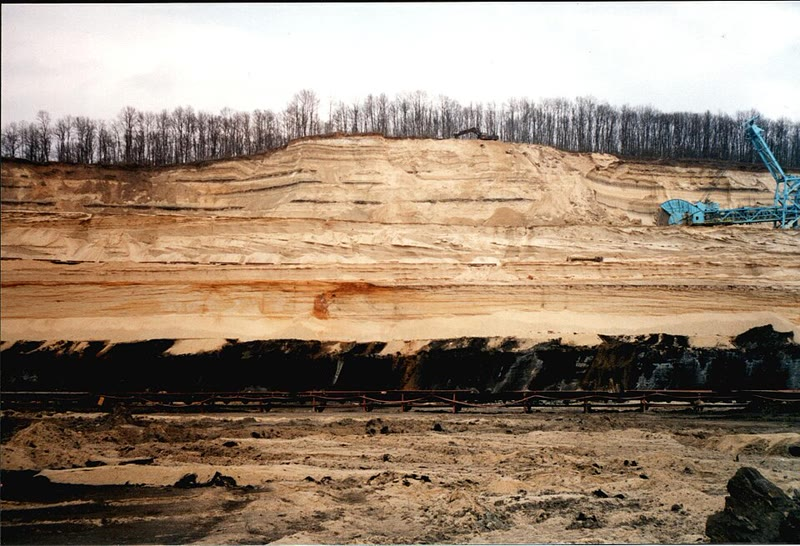
\includegraphics[height=4.0cm]{images/book2/g11-usgs-lignite-bed.jpg}};
\end{tikzpicture}

\medskip
\makebox[0.32\linewidth]{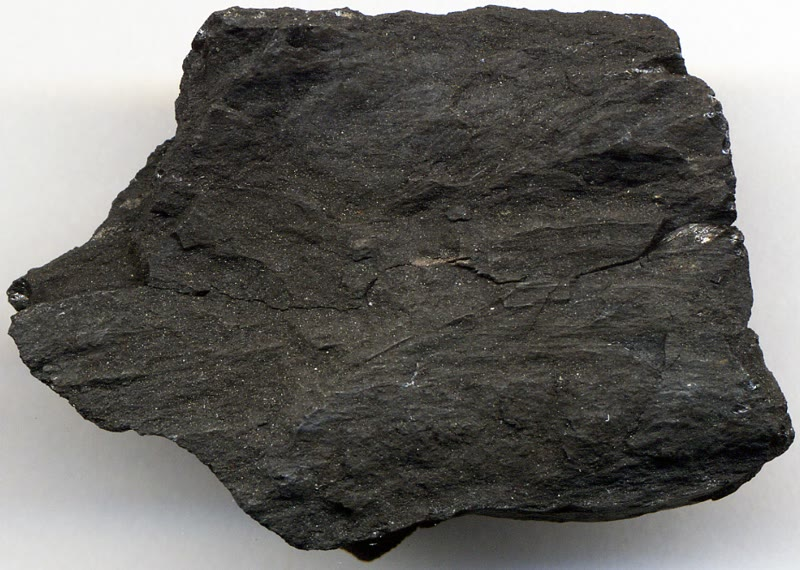
\includegraphics[height=3.2cm]{images/book2/g11-stjohn-lignite.jpg}}\hfill
\makebox[0.32\linewidth]{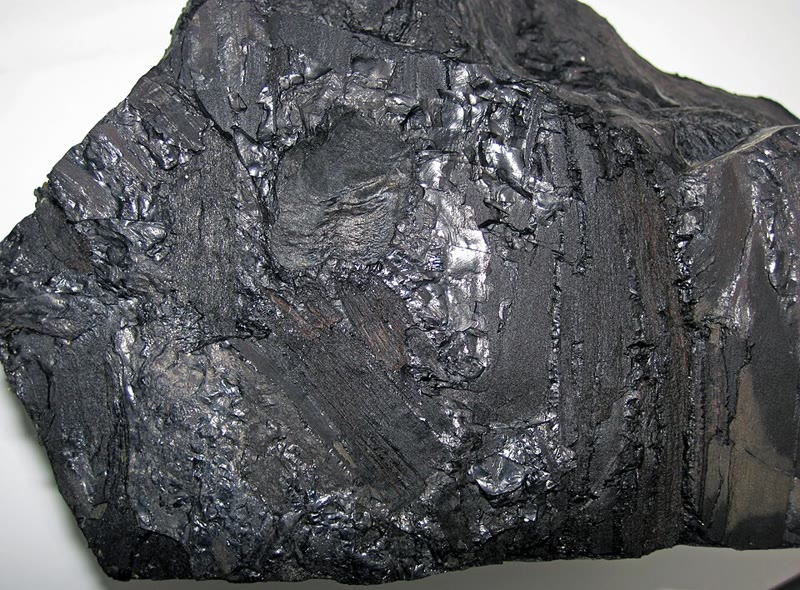
\includegraphics[height=3.2cm]{images/book2/g11-stjohn-bituminous.jpg}}\hfill
\makebox[0.32\linewidth]{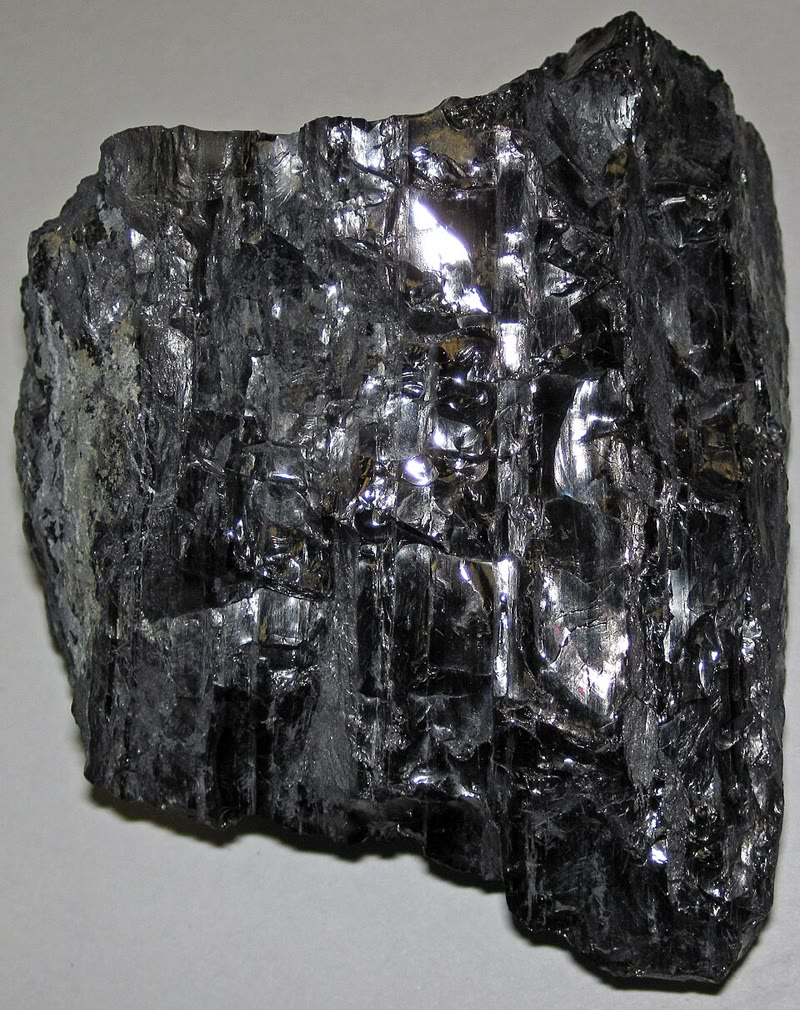
\includegraphics[height=3.2cm]{images/book2/g11-stjohn-anthracite.jpg}}

{\small في الأعلى يسارًا: محتوى الكربون في \omterm{def:g11:fossil-fuel-geology:coal}{رتب الفحم}. البيانات: إدارة
معلومات الطاقة الأمريكية. في الأعلى يمينًا: طبقة من الليغنيت، هي الشريط الأسود
تحت رمال فاتحة، مكشوفة في منجم في رومانيا؛ الصورة: هيئة المسح
الجيولوجي الأمريكية (ملك عام). في الأسفل، من اليمين: الليغنيت، عرضه نحو \qty{4.5}{cm}،
بني مسود وباهت؛ \omterm{def:g11:fossil-fuel-geology:coal}{والفحم} البيتوميني، وفيه قطع نباتية
مسطحة؛ والأنثراسيت، أسود زجاجي. الصور: جيمس سانت~جون
(\babelsublr{CC~BY~2.0}).}
\end{omfigure}
% ledger: eia:coal-carbon, photo:g11-lignite-bed, photo:g11-coal-ranks

يفقد الخث معظم حجمه في الطريق. ففي طبقة \omterm{def:g11:fossil-fuel-geology:coal}{فحم} في وسط يوتا،
تعطي مقارنة الخث الذي اقتطعته قناة نهرية قديمة \omterm{def:g11:fossil-fuel-geology:coal}{بالفحم} المفقود
بجانبها نسبة بين السمكين قدرها نحو $11{:}1$: فكل متر من ذلك
\omterm{def:g11:fossil-fuel-geology:coal}{الفحم} البيتوميني كان يومًا نحو أحد عشر مترًا من الخث.
% ledger: ryer80:peat-coal

\section{تمارين}

\begin{exercise}[$\star$]\label{exo:g11:fossil-fuel-geology:1}
رتّب الخطوات التي تقود من العوالق إلى النفط في \omterm{def:g11:fossil-fuel-geology:trap}{المصيدة}: \omterm{def:g11:fossil-fuel-geology:migration}{الهجرة}؛
\omterm{def:g11:fossil-fuel-geology:oil-window}{النضج} في \omterm{def:g11:fossil-fuel-geology:oil-window}{نافذة النفط}؛ الدفن تحت رواسب أحدث؛ تستقر العوالق الميتة
على قاع بحر فقير بالأكسجين؛ يتجمع النفط تحت \omterm{def:g11:fossil-fuel-geology:reservoir}{صخر حاجز}؛ تصير المادة
العضوية كيروجينًا في وحل.
\end{exercise}

\begin{exercise}[$\star$]\label{exo:g11:fossil-fuel-geology:2}
لكل صخر، قل هل هو على الأرجح \omterm{def:g11:fossil-fuel-geology:source-rock}{صخر مصدر} أم \omterm{def:g11:fossil-fuel-geology:reservoir}{صخر خازن}
أم \omterm{def:g11:fossil-fuel-geology:reservoir}{صخر حاجز}: (1) سجيل داكن غني بالمادة العضوية؛ (2) حجر رملي حسن
الفرز مسامه متصلة؛ (3) طبقة من الملح؛ (4) حجر طيني بلا
مادة عضوية؛ (5) حجر جيري مليء بالتجاويف المفتوحة.
\end{exercise}

\begin{exercise}[$\star$]\label{exo:g11:fossil-fuel-geology:3}
في حوض، السطح عند \qty{10}{\degreeCelsius} \omterm{def:g11:lithosphere-asthenosphere:geotherm}{والتدرج الحراري
الأرضي} \qty{25}{\degreeCelsius/km}. بين أي عمقين تقع \omterm{def:g11:fossil-fuel-geology:oil-window}{نافذة
النفط}؟ وما سمكها؟
\end{exercise}

\begin{exercise}[$\star$]\label{exo:g11:fossil-fuel-geology:4}
(1) رتّب الليغنيت والأنثراسيت \omterm{def:g11:fossil-fuel-geology:coal}{والفحم} البيتوميني والخث بحسب \omterm{def:g11:fossil-fuel-geology:coal}{الرتبة}
تصاعديًا. (2) أيها أعلى محتوى من الكربون؟ (3) أيها تكوّن على
أكبر عمق وأعلى درجة حرارة؟
\end{exercise}

\begin{exercise}[$\star$]\label{exo:g11:fossil-fuel-geology:5}
(1) لماذا يقع الغاز في \omterm{def:g11:fossil-fuel-geology:trap}{المصيدة} فوق النفط، والنفط فوق الماء؟ (2) لماذا
يجب أن يكون الصخر الذي فوق \omterm{def:g11:fossil-fuel-geology:reservoir}{الصخر الخازن} كتيمًا؟ سمّ صخرين يصلحان
صخرين حاجزين.
\end{exercise}

\begin{exercise}[$\star\star$]\label{exo:g11:fossil-fuel-geology:6}
حوضان لهما درجة حرارة السطح نفسها، \qty{15}{\degreeCelsius}.
للحوض A تدرج قدره \qty{20}{\degreeCelsius/km}، وللحوض B
\qty{40}{\degreeCelsius/km}. (1) احسب عمقي أعلى \omterm{def:g11:fossil-fuel-geology:oil-window}{نافذة النفط} وقاعدتها
في كل منهما. (2) يقع \omterm{def:g11:fossil-fuel-geology:source-rock}{صخر مصدر} على عمق \qty{2}{km} في كلا
الحوضين. فماذا يصنع في كل منهما؟ (3) في أي حوض يجب أن تنزل البئر أعمق
لتجد نفطًا تكوّن في موضعه؟
\end{exercise}

\begin{exercise}[$\star\star$]\label{exo:g11:fossil-fuel-geology:7}
خذ النسبة $11{:}1$ المقيسة في وسط يوتا بين سمك
الخث وسمك \omterm{def:g11:fossil-fuel-geology:coal}{الفحم} الذي صار إليه. (1) ما سمك الخث الذي صنع طبقة \omterm{def:g11:fossil-fuel-geology:coal}{فحم}
سمكها \qty{3}{m}؟ (2) لنفترض أن الخث تراكم بمعدل \qty{1}{mm} في السنة.
فكم استغرق تراكمه؟ (3) لماذا لا بد أن المستنقع كان يهبط
طوال ذلك الزمن؟
\end{exercise}

\begin{exercise}[$\star\star$]\label{exo:g11:fossil-fuel-geology:8}
استعمل مخطط تاريخ الدفن لحوض ميرو (السطح عند
\qty{20}{\degreeCelsius}، والتدرج \qty{30}{\degreeCelsius/km}). كان \omterm{def:g11:fossil-fuel-geology:source-rock}{الصخر المصدر}
على عمق \qty{1.2}{km} قبل 120 مليون سنة، و\qty{2.3}{km} قبل 95
مليون سنة، و\qty{4.0}{km} قبل 20 مليون سنة. (1) احسب
درجة حرارته في كل تاريخ. (2) في كل تاريخ، هل كان غير ناضج، أم في \omterm{def:g11:fossil-fuel-geology:oil-window}{نافذة
النفط}، أم في \omterm{def:g11:fossil-fuel-geology:oil-window}{نافذة الغاز}؟
\end{exercise}

\begin{exercise}[$\star\star$]\label{exo:g11:fossil-fuel-geology:9}
يكوّن سطح حجر رملي خازن قوسًا تقع قمته على عمق \qty{2400}{m}؛
وأعمق خط تسوية منغلق له عند \qty{2580}{m}. وبئر عند القمة
تجد الغاز حتى \qty{2450}{m}، ثم النفط. (1) ما أكبر ارتفاع
لعمود يمكن أن تحتجزه \omterm{def:g11:fossil-fuel-geology:trap}{المصيدة}؟ (2) إذا كانت \omterm{def:g11:fossil-fuel-geology:trap}{المصيدة} ممتلئة، فما سمك النفط؟
(3) النفط والغاز اللذان يواصلان الوصول بعد امتلاء \omterm{def:g11:fossil-fuel-geology:trap}{المصيدة}: إلى أين
يذهبان؟
\end{exercise}

\begin{exercise}[$\star\star$]\label{exo:g11:fossil-fuel-geology:10}
حين لا يتوفر أي قياس \omterm{def:g11:fossil-fuel-geology:source-rock}{للكيروجين}، اعتاد جيولوجيو النفط أن يعدّوا
\omterm{def:g11:fossil-fuel-geology:source-rock}{الصخر المصدر} المدفون تحت أكثر من \qty{3}{km} من الصخور ناضجًا.
ومع سطح عند \qty{20}{\degreeCelsius}: (1) أي تدرج يجعل
\qty{3}{km} عند أعلى \omterm{def:g11:fossil-fuel-geology:oil-window}{نافذة النفط}؟ وعند قاعدتها؟ (2) مع
التدرجات المقيسة في الآبار، من 25 إلى \qty{34}{\degreeCelsius/km}،
أين يقع \qty{3}{km}؟ وهل القاعدة معقولة؟
\end{exercise}

\begin{exercise}[$\star\star$]\label{exo:g11:fossil-fuel-geology:11}
ثلاث عينات \omterm{def:g11:fossil-fuel-geology:coal}{فحم} تحوي \qty{30}{\percent} و\qty{70}{\percent}
و\qty{92}{\percent} من الكربون. (1) اذكر \omterm{def:g11:fossil-fuel-geology:coal}{رتبة} كل منها. (2) باستعمال
الأعماق ودرجات الحرارة الواردة في الدرس، أيها دُفن أعمق؟
(3) لليغنيت مظهر باهت بني مسود؛ فكيف يبدو الأنثراسيت؟
\end{exercise}

\begin{exercise}[$\star\star\star$]\label{exo:g11:fossil-fuel-geology:12}
بين 120 و95 مليون سنة مضت، تراكم \qty{1100}{m} من الوحل في
حوض ميرو. (1) احسب معدل الدفن بالأمتار في كل مليون سنة.
(2) مع تدرج قدره \qty{30}{\degreeCelsius/km}، بكم درجة
سخن \omterm{def:g11:fossil-fuel-geology:source-rock}{الصخر المصدر} في كل مليون سنة؟ (3) لو استمر هذا المعدل، فكم
كان سيستغرق \omterm{def:g11:fossil-fuel-geology:source-rock}{الصخر المصدر} ليعبر \omterm{def:g11:fossil-fuel-geology:oil-window}{نافذة النفط} كلها؟ (4) يعطي
النموذج نحو 66 مليون سنة. فلماذا أطول؟
\end{exercise}

\begin{exercise}[$\star\star\star$]\label{exo:g11:fossil-fuel-geology:13}
في حوض ميرو، كان \omterm{def:g11:fossil-fuel-geology:source-rock}{الصخر المصدر} في \omterm{def:g11:fossil-fuel-geology:oil-window}{نافذة النفط} من نحو 117
إلى نحو 51 مليون سنة مضت، وتكوّنت الطية المحدبة التي تحتجز النفط
قبل 80 مليون سنة. (1) افترض أن \omterm{def:g11:fossil-fuel-geology:source-rock}{الصخر المصدر} صنع النفط بمعدل ثابت
ما دام في النافذة. فما الكسر من نفطه الذي تكوّن بعد وجود
\omterm{def:g11:fossil-fuel-geology:trap}{المصيدة}؟ (2) ماذا حلّ بالباقي؟ (3) لو تكوّنت الطية المحدبة قبل 40
مليون سنة، فماذا كانت ستحتجز؟
\end{exercise}

\begin{exercise}[$\star\star\star$]\label{exo:g11:fossil-fuel-geology:14}
خذ تاريخ دفن حوض ميرو (\cref{exo:g11:fossil-fuel-geology:8}:
\qty{0.4}{km} قبل 150 مليون سنة، و\qty{1.2}{km} قبل 120، و\qty{2.3}{km}
قبل 95، و\qty{3.0}{km} قبل 66، والعمق يزداد بانتظام فيما بينها)، لكن في
حوض أسخن: التدرج \qty{40}{\degreeCelsius/km}، والسطح عند
\qty{20}{\degreeCelsius}. (1) احسب عمقي أعلى \omterm{def:g11:fossil-fuel-geology:oil-window}{نافذة النفط} وقاعدتها.
(2) احسب العمرين اللذين دخل عندهما \omterm{def:g11:fossil-fuel-geology:source-rock}{الصخر المصدر} النافذة
وغادرها. (3) لا تزال الطية المحدبة تتكوّن قبل 80 مليون سنة. فهل
تحتجز نفطًا؟ وغازًا؟
\end{exercise}

\begin{exercise}[$\star\star\star$]\label{exo:g11:fossil-fuel-geology:15}
طبقة من الأنثراسيت من العصر الكربوني تتكشف الآن على السطح. وقد
انتهى العصر الكربوني قبل نحو 299 مليون سنة. (1) باستعمال الأعماق الواردة
في الدرس، ما أدنى عمق دُفنت إليه الطبقة؟ (2) مع سطح عند
\qty{15}{\degreeCelsius} وتدرج قدره \qty{30}{\degreeCelsius/km}،
ما درجة الحرارة التي بلغتها على ذلك العمق؟ وهل تتفق مع
درجة الحرارة المذكورة للأنثراسيت؟ (3) ماذا حدث للصخور التي
كانت فوقها؟ أعط حدًا أدنى لمتوسط المعدل، بالمليمترات في
السنة، بافتراض أن كل ذلك حدث بعد العصر الكربوني.
\end{exercise}

\section{مسألة: متى صنع الصخر المصدر النفط؟}

\begin{problem}[{مسألة نهاية الأسبوع --- تأريخ نفط حوض مُتخيَّل}]
\label{pb:g11:fossil-fuel-geology:1}
% values (oil_window.py): enter_oil_Ma 116.97, leave_oil_Ma 51.238, T_max 140, T_today 125,
% after_trap_frac 0.43757; ledger ics:base.Jurassic, ics:base.Cretaceous, earle:*, magoon00:tps
بئر محفورة عبر قمة طية محدبة في حوض ميرو، وهو حوض
مُتخيَّل، تعبر الطبقات التي تحتها. وهذه الطبقات، المؤرخة بأحافيرها،
تسجّل كيف امتلأ الحوض. بدءًا من الأقدم:
\begin{center}
\small
\begin{tabular}{|l|l|l|}
\hline
\textbf{الفترة (بملايين السنين قبل الحاضر)} & \textbf{السمك} & \textbf{الصخور} \\
\hline
165 إلى 150 & \qty{400}{m} & سجيل أسود غني بالمادة العضوية، ثم حجر طيني \\
150 إلى 120 & \qty{800}{m} & حجر رملي مسامي \\
120 إلى 95 & \qty{1100}{m} & حجر طيني \\
95 إلى 66 & \qty{700}{m} & طباشير \\
66 إلى 35 & \qty{700}{m} & رمال وطين \\
35 إلى 20 & \qty{300}{m} & رمال \\
20 إلى اليوم & \qty{-500}{m} & \foreignlanguage{arabic}{نهوض: تآكل الجزء الأعلى البالغ \babelsublr{\qty{500}{m}}} \\
\hline
\end{tabular}
\end{center}
السطح عند \qty{20}{\degreeCelsius} \omterm{def:g11:lithosphere-asthenosphere:geotherm}{والتدرج الحراري الأرضي}
\qty{30}{\degreeCelsius/km}، وكلاهما يُعَدّ ثابتًا. وتحتفظ الطبقات بسمكها
بعد ترسبها (يُهمَل الانضغاط). وتكوّنت الطية المحدبة قبل 80
مليون سنة. تتبّع السجيل الأسود الذي في القاعدة، الذي ترسب قبل 165 مليون
سنة.

\medskip
\noindent\textbf{الجزء الأول --- الصخور.}
\begin{enumerate}
  \item أي طبقة هي \omterm{def:g11:fossil-fuel-geology:source-rock}{الصخر المصدر}، وأيها \omterm{def:g11:fossil-fuel-geology:reservoir}{الصخر الخازن}، وأيها \omterm{def:g11:fossil-fuel-geology:reservoir}{الصخر الحاجز}؟
  \item ما الذي جعل السجيل الأسود غنيًا بالمادة العضوية؟
  \item امتد الجوراسي من نحو \num{201.4} إلى \num{143.1} مليون
        سنة مضت. ففي أي عصر ترسب \omterm{def:g11:fossil-fuel-geology:source-rock}{الصخر المصدر}؟
        والحجر الرملي؟
  \item ما \omterm{def:g11:fossil-fuel-geology:source-rock}{الكيروجين}؟ ولماذا لا يصنع السجيل الأسود نفطًا عند
        السطح؟
  \item ما سمك الصخور التي تعلو \omterm{def:g11:fossil-fuel-geology:source-rock}{الصخر المصدر} اليوم؟
\end{enumerate}

\medskip
\noindent\textbf{الجزء الثاني --- الدفن بدلالة الزمن.}
\begin{enumerate}[resume]
  \item احسب عمق \omterm{def:g11:fossil-fuel-geology:source-rock}{الصخر المصدر} قبل 150 و120 و95 و66 و35 و20
        مليون سنة، واليوم.
  \item احسب معدل الدفن، بالأمتار في كل مليون سنة، خلال
        كل فترة من الفترات الست الأولى.
  \item متى كان \omterm{def:g11:fossil-fuel-geology:source-rock}{الصخر المصدر} في أعمق موضع له، وعلى أي عمق؟
  \item لماذا تناقص عمقه خلال ملايين السنين العشرين الأخيرة؟
  \item ما عمق قاعدة الحجر الرملي اليوم؟
\end{enumerate}

\medskip
\noindent\textbf{الجزء الثالث --- درجة الحرارة بدلالة الزمن.}
\begin{enumerate}[resume]
  \item احسب درجة حرارة \omterm{def:g11:fossil-fuel-geology:source-rock}{الصخر المصدر} في كل تاريخ من تواريخ
        السؤال~6.
  \item بين أي عمقين تقع \omterm{def:g11:fossil-fuel-geology:oil-window}{نافذة النفط} في هذا الحوض؟
  \item بين أي تاريخين من تواريخ السؤال~6 تجاوز \omterm{def:g11:fossil-fuel-geology:source-rock}{الصخر المصدر}
        \qty{60}{\degreeCelsius}؟
  \item بافتراض أن عمقه ازداد بانتظام في تلك الفترة، احسب العمر
        الذي بلغ عنده \qty{60}{\degreeCelsius}.
  \item احسب بالطريقة نفسها متى بلغ \qty{120}{\degreeCelsius}.
\end{enumerate}

\medskip
\noindent\textbf{الجزء الرابع --- إلى داخل النافذة، والمصيدة.}
\begin{enumerate}[resume]
  \item ما أعلى درجة حرارة بلغها؟ وماذا يصنع
        اليوم؟
  \item ماذا حلّ بالنفط المتكوّن قبل وجود الطية المحدبة؟
  \item بافتراض أن النفط تكوّن بمعدل ثابت ما دام \omterm{def:g11:fossil-fuel-geology:source-rock}{الصخر المصدر} في
        النافذة، فما الكسر منه الذي تكوّن بعد وجود الطية المحدبة؟
  \item أي الموائع تتوقع البئر عند قمة الطية المحدبة،
        وبأي ترتيب من الأعلى؟
  \item استنتج: متى دخل \omterm{def:g11:fossil-fuel-geology:source-rock}{الصخر المصدر} \omterm{def:g11:fossil-fuel-geology:oil-window}{نافذة النفط}؟
\end{enumerate}
\end{problem}
